% Pacotes
\documentclass[12pt]{article}
\usepackage{adjustbox}
\usepackage[utf8]{inputenc}
\usepackage{amsmath}
\usepackage{hyperref}
\usepackage{sbc-template}
\usepackage{fancyvrb}
\usepackage{amsfonts}
\usepackage{amsmath}
\usepackage{pdfpages}
\usepackage{graphicx,url}


\sloppy

\title{Relatório - Xadrez em Racket}

\author{Ricardo Henrique Brunetto\inst{1}}


\address{Departamento de Informática -- Universidade Estadual de Maringá (UEM)\\
	Maringá -- PR -- Brasil
	\email{ra94182@uem.br}
}

\begin{document}

	\maketitle

	{\resumo{}}

  \section{Introdução}
	O presente documento é um relatório do desenvolvimento de um jogo de Xadrez na
	linguagem funcional Racket para a disciplina 6902 - Paradigma de Programação Lógica
	e Funcional, ministrada pelo professor Dr. Wagner Igarashi para a turma de 2015
	de Bacharelado em Ciência da Computação pela Universidade Estadual de Maringá.

	Neste relatório serão abordadas seções conforme socilitado na especificação do trabalho,
	que pode ser encontrada em anexo a este documento.

	\section{O Jogo}

	O jogo foi desenvolvido em Racket com uso do editor de textos Atom e da IDE DrRacket.
	Fazer-se-á uma breve explanação a respeito das regras do jogo e de seu funcionamento.
	Em seguida, serão apresentados os aspectos avaliativos, conforme solicitado.

	Em suma, o jogo segue as regras de um Xadrez convencional, sem, no entanto, movimentos especiais.
	Isso significa que o jogador não será capaz de aplicar técnicas como \textit{The Rock}. Não há,
	também, avaliação quanto ao xeque (ou xeque mate).

	Quanto à movimentação das peças, seguem-se as regras-padrão do jogo.

	\subsection{Variáveis do Jogo}
	O jogo foi construído utilizando a biblioteca \verb|universe|, o que requireu que fosse desenvolvida
	uma estrutura de \verb|world| \cite{racketdoc}. Internamente, a cada interação do usuário com o jogo,
	é criada uma nova estrutura de \verb|world|.

	Dessa forma, desenvolveu-se a esturuta \textit{jogada}. Essa estrutura tem por objetivo simular um
	\verb|world|, ou seja, encapsular todas as variáveis que se alteram entre as jogadas.
\begin{Verbatim}[fontsize=\footnotesize]
	(struct jogada (tab jogador king ptsB ptsP))
\end{Verbatim}
Dentre as variáveis, encontram-se:
\begin{itemize}
	\item \verb|tab| que se refere a um Tabuleiro (definido posteriormente) $\{mutable-array\}$;
	\item \verb|jogador| que se refere ao Jogador que está atualmente jogando (definido posteriormente) $\{jogador\}$;
	\item \verb|king| que se refere à variável que atesta que ambos reis estão vivos (0) ou algum está morto (1) $\{number\}$;
	\item \verb|ptsB| que se refere aos pontos do jogador das peças brancas $\{number\}$;
	\item \verb|ptsP| que se refere aos pontos do jogador das peças pretas $\{number\}$.
\end{itemize}

As principais estruturas do jogo são \verb|peca|, \verb|pos| e \verb|tabuleiro|.
\begin{itemize}
		\item \verb|peca| é uma \textbf{peça do tabuleiro}, devendo possuir:
			\subitem \verb|id|: identificação única inteira $id$ $\{number\}$;
			\subitem \verb|tipo|: informa a classe da peça, podendo variar entre \textbf{peao, torre, cavalo, bispo, rainha, rei} $\{string\}$.
			\subitem \verb|cor|: informa a cor da peça (pertinência ao jogador que a controla) $\{color\}$.
			\subitem \verb|imagem|: informa o bitmap da peça (interface gráfica) $\{bitmap\}$.
		\item \verb|pos| é uma \textbf{posição do tabuleiro}, devendo possuir:
			\subitem \verb|x| e \verb|y|: coordenadas inteiras, onde $0 \leq x, y \leq 7$ $\{number\}$;
			\subitem \verb|destinavel|: um booleando para informar se a posição é um destino válido de outra $\{boolean\}$;
			\subitem \verb|peca|: que representa a peça que ocupa a posição (pode ser \verb|empty|) $\{peca\}$.
		\item \verb|tabuleiro| representa o próprio \textbf{tabuleiro}, sendo um $array\; 8\times8$ de \verb|pos|, cada qual com sua \verb|peca|. $\{mutable-array\}$;
\end{itemize}
\begin{Verbatim}[fontsize=\footnotesize]
(struct peca (id tipo cor imagem) #:transparent #:mutable)
(struct pos (x y destinavel peca) #:transparent #:mutable)
(define tabuleiro (mutable-array #[#[A8 B8 C8 D8 E8 F8 G8 H8]
                                   #[A7 B7 C7 D7 E7 F7 G7 H7]
                                   #[A6 B6 C6 D6 E6 F6 G6 H6]
                                   #[A5 B5 C5 D5 E5 F5 G5 H5]
                                   #[A4 B4 C4 D4 E4 F4 G4 H4]
                                   #[A3 B3 C3 D3 E3 F3 G3 H3]
                                   #[A2 B2 C2 D2 E2 F2 G2 H2]
                                   #[A1 B1 C1 D1 E1 F1 G1 H1]]))
\end{Verbatim}
onde cada $Kij$, com $K\in\{A,\dots,H\}\,i,j\in\{1,\dots,8\}$ é uma instância definida de \verb|pos|.

Para controle dos jogadores, desenvolveu-se uma estrutura \verb|jogador| que armazena uma \textit{string} $nome$ e uma $color$ $cor$.
Por definição, apenas dois jogadores podem participar de uma partida.
\begin{Verbatim}[fontsize=\footnotesize]
	(struct jogador (nome cor) #:mutable)
\end{Verbatim}

Além disso, são definidas as seguintes variáveis, que auxiliam na construção de uma \verb|jogada| ($World$):
\begin{Verbatim}[fontsize=\footnotesize]
(define ranking empty)
(define jogadorIA1 empty) ;Define quem é o jogador IA 1
(define jogadorIA2 empty) ;Define quem é o jogador IA 2
(define jogadorHumano1 empty) ;Define quem é o jogador Humano 1
(define jogadorHumano2 empty) ;Define quem é o jogador Humano 2
(define nomeJogador1 empty) ;Define o nome do jogador humano 1
(define nomeJogador2 empty) ;Define o nome do jogador humano 2
;Variável para controlar os cliques (selecionar origem = 0 / selecionar destino = 1)
(define select 0)
(define movimentos 0) ;Variável para contar os movimentos
(define jogador-atual empty);Define quem é o jogador atual
;Lista de possibilidades de locomoção temporárias
(define possibilidades-temporarias empty)
;Posição de origem (de onde um jogador deseja fazer o movimento)
(define posicao-origem empty)
;Variável que atesta que ambos reis estão vivos (0) ou algum está morto (1)
(define king-is-dead 0)
(define pts-branco 0) ;Placar do jogador branco
(define pts-preto 0) ;Placar do jogador preto
\end{Verbatim}

A movimentação das peças é realizada através de \textbf{expressões Lambda}. São definidas duas funções
principais para a definir as possibilidades de destino das peças: \verb|unitario|, que
Aplica uma única vez (unitário) as funções para cada possibilidade, filtrando com uma função de validação; e
\verb|get-recursivo-possibilidades|, que aplica recursivamente as funções em Lfuncoes para cada possibilidade.

Em suma, ambas retornam uma lista de posições (\verb|pos|) que determinada peça em uma posição $posX$ pode ter como destino.
Para tanto, recebem uma Lista de Funções (\verb|Lfuncoes|) a ser aplicada nas coordenadas de $posX$. A diferença está no fato
de que a \verb|get-unitario-possibilidades| aplica uma única vez cada função e as valida com uma função de validação \verb|fval|,
enquanto a \verb|get-recursivo-possibilidades| aplica cada função em \verb|Lfuncoes| recursivamente para cada posição gerada.

Esse modelo é, na verdade, uma abstração do comportamento do cálculo das possibilidades para as peças. Uma peça como um peão, por exmeplo,
faz uso de um cálculo unitário (verifica os arredores, apenas) enquanto a torre, por outro lado, faz uso de um cálculo recursivo (verifica
os arredores e os arredores dos arredores, sucessivamente, até encontrar uma posição considerada inválida). Os critérios para determinar qual
a próxima posição da torre difere dos critério de determinação da próxima posição do bispo, por exemplo. Nesse ínterim entra a lista de expressões
\textbf{lambda}. Dessa forma, tem-se:

\begin{Verbatim}[fontsize=\footnotesize]
; Lista de funções para as possibilidades de locomoção do Cavalo
(define Lf-Cavalo (list (list (lambda(x)(sub1 x))  (lambda(y)(+ y 2)))
                        (list (lambda(x)(add1 x))  (lambda(y)(+ y 2)))
                        (list (lambda(x)(+ x 2))   (lambda(y)(add1 y)))
                        (list (lambda(x)(- x 2))   (lambda(y)(add1 y)))
                        (list (lambda(x)(- x 2))   (lambda(y)(sub1 y)))
                        (list (lambda(x)(+ x 2))   (lambda(y)(sub1 y)))
                        (list (lambda(x)(add1 x))  (lambda(y)(- y 2)))
                        (list (lambda(x)(sub1 x))  (lambda(y)(- y 2)))))
; Lista de funções para as possibilidades de locomoção do Bispo
(define Lf-Bispo  (list (list (lambda(x)(sub1 x))  (lambda(y)(add1 y)))
                        (list (lambda(x)(sub1 x))  (lambda(y)(sub1 y)))
                        (list (lambda(x)(add1 x))  (lambda(y)(add1 y)))
                        (list (lambda(x)(add1 x))  (lambda(y)(sub1 y)))))
; Lista de funções para as possibilidades de locomoção da Torre
(define Lf-Torre  (list (list (lambda(x)(sub1 x))  (lambda(y)y))
                        (list (lambda(x)(add1 x))  (lambda(y)y))
                        (list (lambda(x)x)         (lambda(y)(add1 y)))
                        (list (lambda(x)x)         (lambda(y)(sub1 y)))))
; Lista de funções para as possibilidades de locomoção do Peao Preto
(define Lf-Peao-P (list (list (lambda(x)(add1 x))  (lambda(y)(add1 y)))
                        (list (lambda(x)(add1 x))  (lambda(y)y))
                        (list (lambda(x)(add1 x))  (lambda(y)(sub1 y)))))
; Lista de funções para as possibilidades de locomoção do Peao Branco
(define Lf-Peao-B (list (list (lambda(x)(sub1 x))  (lambda(y)(add1 y)))
                        (list (lambda(x)(sub1 x))  (lambda(y)y))
                        (list (lambda(x)(sub1 x))  (lambda(y)(sub1 y)))))
; Lista de funções para as possibilidades de locomoção do Rei
(define Lf-Rei    (list (list (lambda(x)(sub1 x))  (lambda(y)y))
                        (list (lambda(x)(sub1 x))  (lambda(y)(add1 y)))
                        (list (lambda(x)(sub1 x))  (lambda(y)(sub1 y)))
                        (list (lambda(x)x)         (lambda(y)(add1 y)))
                        (list (lambda(x)x)         (lambda(y)(sub1 y)))
                        (list (lambda(x)(add1 x))  (lambda(y)(sub1 y)))
                        (list (lambda(x)(add1 x))  (lambda(y)y))
                        (list (lambda(x)(add1 x))  (lambda(y)(add1 y)))))
\end{Verbatim}

	\subsection{Jogadores e Modos de Jogo}
	Foi desenvolvido o jogo de Xadrez com três modos de jogo:
	\begin{itemize}
		\item Humano vs. Humano
		\item Humano vs. Computador
		\item Computador vs. Computador
	\end{itemize}

	O usuário seleciona o modo de jogo através de uma interface gráfica:
	\begin{figure}[h]
		\centering
		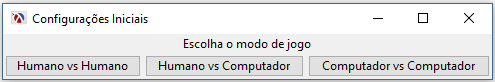
\includegraphics[scale = 0.7]{escolha.png}
		\caption{Escolha do modo de jogo}
	\end{figure}

	Para cada jogador humano, há uma janela de seleção:
	\begin{figure}[h]
		\centering
		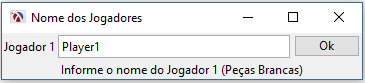
\includegraphics[scale = 0.7]{player1.png}
		\caption{Obtenção do nome do jogador humano 1}
	\end{figure}
	\begin{figure}[h]
		\centering
		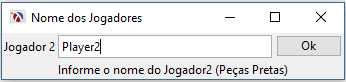
\includegraphics[scale = 0.7]{player2.png}
		\caption{Obtenção do nome do jogador humano 2}
	\end{figure}

	Ao contrário do restante do jogo, estas janelas são construídas com a biblioteca \verb|racket/gui|.

	\subsection{Interface Gráfica do Jogo}

	 Após a seleção do modo de jogo, a interface gráfica do jogo é desenhada na tela, conforme ilustrado por \ref{lblfig}.
	 \begin{figure}[h]
	 	\centering
	 	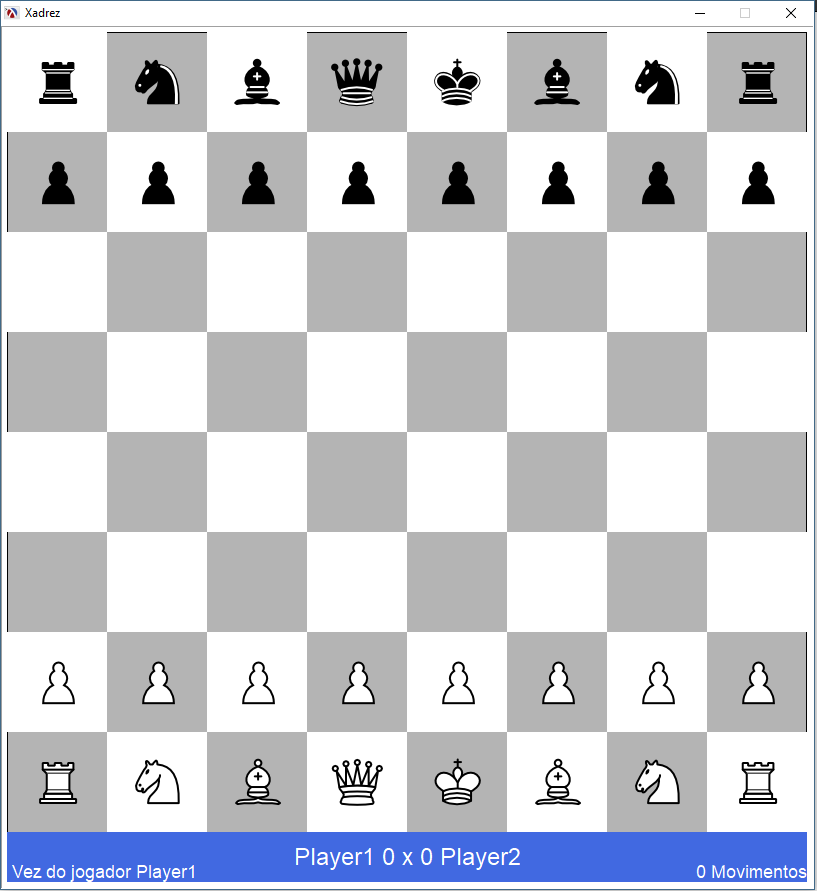
\includegraphics[scale = 0.5]{screen.png}
		\label{lblfig}
	 	\caption{Interface Gráfica do Jogo}
	 \end{figure}

	Um destaque especial para o momento em que o jogador Humano seleciona uma determinada peça e as possibilidades
	são desenhadas com pontos verdes centrais em cada posição conforme ilustrado por \ref{fig2}.

	\begin{figure}[h]
		\centering
		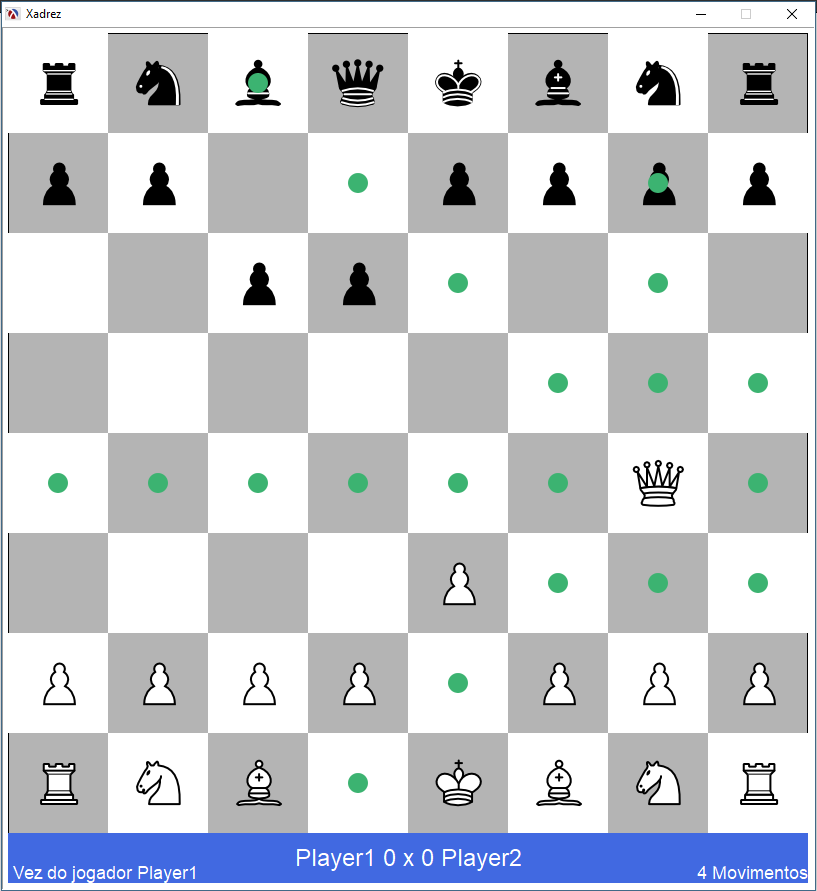
\includegraphics[scale = 0.5]{possibilidades.png}
		\caption{Possibilidades de Locomoção da Rainha Branca}
		\label{fig2}
	\end{figure}

	\subsection{Placar Final}
	Durante o jogo, há uma barra inferior que mostra o placar atual. O placar é dado conforme os jogadores consomem peças do
	adversário.

	Cada peça tem para si um peso associado, conforme sua importâcia no tabuleiro. A pontuação final é:
	\begin{itemize}
		\item Peao = 1
		\item Torre = 3
		\item Cavalo = 5
		\item Bispo = 7
		\item Rainha  = 10
		\item Rei  = 49 (soma de todas as peças do oponente + 1)
	\end{itemize}

	Quando o jogo termina, pode-se jogar novamente (nas mesmas configurações iniciais) através da tecla [ENTER]. A figura \ref{fig3}
	mostra a tela final do jogo:
	\begin{figure}[h]
		\centering
		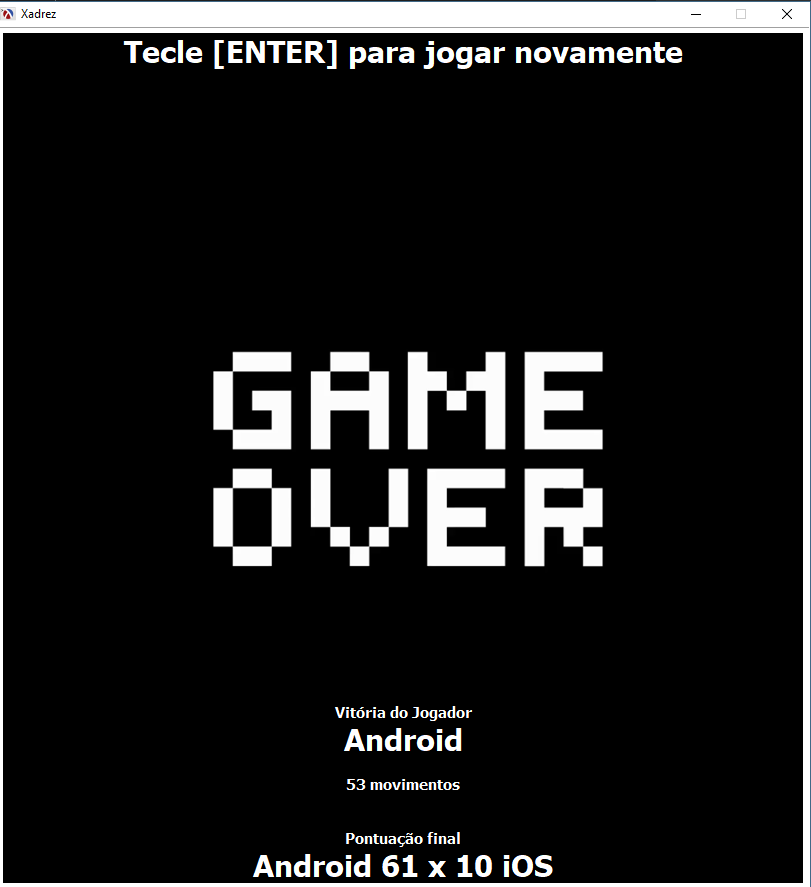
\includegraphics[scale = 0.5]{final.png}
		\caption{Tela de Final de Jogo}
		\label{fig3}
	\end{figure}


	\subsection{Inteligência Artificial}

	A intelência artificial desenvolvida para a resolução do jogo aplica a seguinte heurística:
	\begin{enumerate}
			\item Selecionar aleatóriamente uma peça
			\item Buscar as possibilidades de destino (caso vazio, selecionar outra peça)
			\item Buscar pela posição onde se encontra a peça mais valiosa do jogador (caso não haja, mover-se aleatoriamente).
	\end{enumerate}

	Assim, o computador tenta, dada uma peça aleatória, encontrar a posição que mais tem importância para o adversário.

	Dessa forma, uma partida \textit{Computador vs. Computador} consiste de dois jogadores aplicando tal heurística até que um deles perca o rei.

	\section{Análise do Algoritmo de IA}

	Conforme apresentado na seção anterior, fora desenvolvido um algoritmo para jogar sozinho. Para efeitos de teste, foram executadas
	$40$ partidas no modo \textit{Computador vs. Computador} e analisados dados referentes à:
	\begin{itemize}
		\item \textbf{Quantidade de Movimentos} totais da partida
		\item \textbf{Pontuação do jogador 1}
		\item \textbf{Pontuação do jogador 2}
	\end{itemize}
%
De maneira geral, pôde-se construir a tabela \ref{my-label}:
\begin{table}[]
\centering
\label{my-label}
\begin{tabular}{|l|c|c|c|}
\hline
                         & \textbf{Média} & \textbf{Mediana} & \textbf{Desvio Padrão} \\ \hline
\textbf{Movimentos}      & 63,25          & 49               & 3,256                  \\ \hline
\textbf{Pontos - Branco} & 52,21          & 37               & 2,35                   \\ \hline
\textbf{Pontos - Preto}  & 39,54          & 35               & 5,23                   \\ \hline
\end{tabular}
\caption{Análise dos Dados do algoritmo de IA}
\end{table}

Os resultados altos de \textbf{Movimentos} devem-se principalmente à aleatoriedade na selação das peças, o que
fez o computador perder oportunidades de finalizar o jogo com maior antecedência, em um número menor de movimentos.

	\newpage
	\bibliographystyle{sbc}
	\bibliography{references}

\end{document}
